\documentclass{article}[11 pt]
\usepackage{graphics}
\usepackage{color}
\usepackage{graphicx,subcaption}
\usepackage{amsmath,bbm,amssymb,mathrsfs,bm}
\usepackage{amsthm}
\usepackage{comment}
\usepackage{rotating}
\usepackage{lscape}
\usepackage{enumerate}
\usepackage{fullpage}
\usepackage{hyperref}
\usepackage[usenames,dvipsnames]{xcolor}
\setcounter{secnumdepth}{3}
\begin{document}
\begin{center}	
	\textbf{Mexican Drug War: Have the Military Interventions Increased Violence?}
\end{center}

When we start to approach this problem the first to consider is what data is available to analyze it. We are using the Military interventions listed in a non comprehensive list from may 7,2007 - nov 21, 2010) NEXOS paper: \url{http://www.nexos.com.mx/?P=leerarticulo&Article=1943189 }. %Read this again to use their terminology.

The measure of violence that we are using is homicide rate, Y. This could be debatable, maybe a combined measure of different kinds of crimes would be better.

Assumptions:
\begin{itemize}
	\item SUTVA
	\item Unconfoundedness: a very strong assumption is that we have all the covariates that could affect the homicide rates. In other words that we have all covariates, X, such that given X,  W is independent of Y.
	\item That homicide rates, Y, are an accurate measure of violence. 
\end{itemize}

The main idea is to combine synthetic and propensity score matching to address this question. What are the advantages of doing that? (and what's new?)
The current proposal is to use propensity score matching to create pools of acceptable controls for each treated unit (is there some multiple comparison thing going on here? Probably not, we just cared about the observed imbalances, we are not saying anything else.). Furthermore, to get the synthetic match for treated unit $T_i$ we can choose the weights for the units in it's control pool such that the $Y_1^T,\ldots, Y_{I_i}^{T_i}$ is best matched

\subsection{How to make SUTVA more feasible?}
The main idea is to group neighboring regions that have received military interventions (that have resulted in deaths) in such a way that distances make no interference more reasonable or geographic situation such as lack of highways connecting them \url{http://mx.kalipedia.com/kalipediamedia/geografia/media/200805/11/geomexico/20080511klpgeogmx_4_Ges_SCO.png} or big mountains between them, or closeness to where the crops or smuggling routes are \url{http://utopiaguatemala.files.wordpress.com/2011/11/mexico_routes_in_466.gif} (can we find such data?).
We proposed the following units (the bold names are the ones that actually received an intervention):
\begin{enumerate}
\item \textbf{Tijuana}, Playas de Rosarito, Tecate, Ensenada (Baja California)
\item \textbf{Nogales}, Sáric, Tubutama, Magdalena, Imuris, Santa Cruz (Sonora)
\item \textbf{Madera}*, Temósachic, Casas Grandes, Zaragoza, Gómez Farías, Matachí (Chihuahua) Yécora, Arivechi, Sahuaripa, Nácori Chico, Huachinera, Bacerac, Bacadéhuachi (Sonora)
\item \textbf{Juárez, Chihuahua}, Ascensión, Ahumada, Guadalupe, Praxedis G. Guerrero, Coyame del Socol, Aldama, Aquiles Serdán, Rosales, Satevó, Dr. Belisario Dominguez, Santa Isabel, Riva Palacio, Namiquipa, Buenaventura (Chihuahua)
\item \textbf{Pánuco *}, Pueblo Viejo, Tampico Alto, El Higo, Tempoal, Ozuluama de Mascareñas (Veracruz), \textbf{Tampico}, Ciudad Madero, Altamira, González, El Mante (Tamaulipas), Ebano,Tamuín, San Vicente Tancuayalab (San Luis Potosí)
\item\textbf{ Nuevo Laredo*, Guerrero*, Mier*, Miguel Alemán*, Díaz Ordaz*, Reynosa, Río Bravo, Matamoros*}, Camargo, Valle Hermoso, Méndez, San Fernando (Tamaulipas), Dr. Cos, Anáhuac, Gral. Bravo, China, Vallecillo, Parás, Agualeguas (Nuevo León), \textbf{Melchor Ocampo*}, Los Herreras, Los Aldamas, Gral Treviño, Cerralvo (Nuevo León)
\item\textbf{ Bustamante*}, Villaldama, Mina, Lampazos de Naranjo (Nuevo León), Candela (Coahuila)
\item \textbf{Santa Catarina*, Guadalupe, Juárez*, General Zuazua}, Higueras, Marín, Pesquería, Apodaca, General Escobedo, Carmen,Salinas Victoria, Ciénega de Flores, Cadereyta Jiménez, Santiago, Monterrey, San Pedro Garza García, García, San Nicolás de los Garza, (Nuevo León), Ramos Arizpe, Arteaga (Coahuila)
\item \textbf{Villa de Cos, Fresnillo, Tepetongo*}, Pánuco, Calera, General Enrique Estrada, Jerez , Susticacán, Valparaíso, Sombrerete, Sain Alto, Río Grande, Cañitas de Felipe Pescador, General Francisco R. Murguía, Mazapil, Guadalupe,Villanueva, Monte Escobedo (Zacatecas), Villa de Ramos,  Santo Domingo  (San Luis Potosí), Huejúcar, Santa María de los Ángles (Jalisco)
\item Teúl de González Ortega, Mezquital, Trinidad García de la Cadena, Moyahua de Estrada, Juchipila, Apozol, Santa María de la Paz, Benito Juárez (Zacatecas), Tequila, San Martín de Bolaños (Jalisco)
\itemRincón de Romos, Tepezalá, Cosío, San José de Gracia, Pabellón de Arteaga (Aguascalientes), Cuauhtémoc, Genaro Codina, Luis Moya (Zacatecas)
\itemSinaloa, Badiraguato, Choix, El Fuerte, Ahome, Guasave, Salvador Alvarado, Mocorito, Culiacán (Sinaloa), Guadalupe y Calvo, Morelos (Chihuahua), Tamazula (Durango) Santiago Papasquiaro*, Pueblo Nuevo, Tamazula, Otáez, San Dimas, Nuevo Ideal, Canatlán, Coneto de Comonfort, El Oro, Tepehuanes, Topia, Durango, Canelas,Mezquital (Durango), Huajicori (Nayarit), Rosario, Concordia (Sinaloa)
\itemRosamorada*, Tepic*, Tecuala, Santiago Ixcuinta, Tuxpan, Ruíz, Del Nayar, Acaponeta, Tecuala, San Blas, Xalisco, Santa María del Oro, (Nayarit)
La Piedad*, Numarán, Zináparo, Churintzio, Ecuandureo, Yurécuaro (Michoacán), Pénjamo (Guanajuato), Ayotlán, Degollado  (Jalisco)
Celaya, Cortazar, Salvatierra, Tarimoro, Apaseo el Alto, Apaseo el Grande, Comonfort, Santa Cruz De Juventino Rosas, Villagrán (Guanajuato)
\itemApatzingán, Buenavista, Aguililla, Tumbiscatío, La Huacana, Múgica, Parácuaro, Tancítaro, Tepalcatepec (Michoacán)
Coahuayana*, Aquila, Chinicuilla (Michoacán), Ixtlahacán, Tecomán, Colima (Colima)
\item Taxco*, Teloloapan, Arcelia, San Miguel Totolapan, Acapulco, Ajuchitlán del Progreso, San Marcos, Juan R. Escudero, Tecoanapa ,Chilpancingo de los Bravo, Coyuca de Benítez, Atoyac de Álvarez, Técpan de Galeana, Coyuca de Catalán, Pungarabato, Tlapehuala, Tlalchapa, General Canuto A. Neri, Pedro Ascencio Alquisiras, Ixcateopan de Cuauhtémoc, Tetipac,Pilcaya, Benito Juárez, Buenavista de Cuéllar, Iguala de la Independencia, Cocula, Cuetzala del Progreso, Apaxtla, General Heliodoro Castillo  (Guerrero), Tlatlaya, Amatepec, Sultepec,  Zacualpan (México), Amacuzac,Tetecala, Coatlán del Río(Morelos)

	

There are 2213 municipalities in the initial control pool, and the numbers per treated unit are:
  % latex table generated in R 2.14.0 by xtable 1.6-0 package
% Thu Sep 27 10:40:57 2012
% \begin{table}[ht]
% \begin{center}
% \begin{tabular}{rc|rc}
% 
%   \hline 
%   \textbf{1 }&   5 &\textbf{10} &  10 \\ 
%   \textbf{2} &   5 &\textbf{11} &   8 \\  
%   \textbf{3} &  12 &\textbf{12 }&  27 \\ 
%   \textbf{4} &  15 & \textbf{13} &  11 \\
%   \textbf{5} &  14 & \textbf{14} &   9 \\ 
%   \textbf{6} &  24 & \textbf{15} &   9 \\ 
%   \textbf{7} &   5 &  \textbf{16} &  10 \\ 
%   \textbf{8} &  20 &\textbf{17} &   6 \\ 
%   \textbf{9} &  18 & \textbf{18 }&  35 \\
% \hline
% \end{tabular}
% \end{center}
% \end{table}


% latex table generated in R 2.14.0 by xtable 1.6-0 package
% Thu Sep 27 14:57:21 2012
\begin{table}[ht]
\begin{center}
\begin{tabular}{ccc|ccc}
  \hline
 \textbf{unit}& number of& Date of first &  \textbf{unit}& number of& Date of first \\ 
 & municipalities& intervention& & municipalities& intervention \\ 
  \hline
\textbf{1} &   5 & 2008 &  \textbf{10} &10 & 2009 \\ 
  \textbf{2} &   5 & 2008 &  \textbf{11} & 8 & 2008 \\ 
  \textbf{3} &  12 & 2010* &  \textbf{12} &27 & 2007 \\ 
  \textbf{4} &  15 & 2009 &  \textbf{13} &11 & 2010* \\ 
  \textbf{5} &  14 & 2007 &   \textbf{14} &9 & 2010* \\ 
  \textbf{6} &  24 & 2008 &   \textbf{15} &9 & 2009 \\ 
  \textbf{7} &   5 & 2010* &  \textbf{16} &10 & 2007 \\ 
  \textbf{8} &  20 & 2009 &   \textbf{17} &6 & 2010* \\ 
  \textbf{9} &  18 & 2008 &  \textbf{18} &35 & 2008 \\ 
   \hline
\end{tabular}
\end{center}
\end{table}

Note that for the data that we're working with, all the regions with $*$ are eliminated from the data set since we have no post intervention information. The data collected spans 1990-2010. That leaves us with 205 treated municipalities.

\section{Estimand}
We want to measure the effect of the military interventions in terms of the increase in homicide rates. Following the Rubin Causal Model, let $Y_j(1)$ and $Y_j(0)$ denote the homicide rate of region $j$ one year after it received a military intervention\footnote{We can also estimate the effect two and three years post intervention. However, the uncertainty will increase because there are only three regions with 2007 interventions and an additional six with 2008 interventions.}, and what it would have been at that same point in time if it hadn't received the military intervention. The estimand of interest is the average causal effect of the military intervention for the regions that were intervened. That is $$\tau=\overline{Y}(1)-\overline{Y}(0)=\frac{\sum_j Y_j(1)-Y_j(0)}{J}.$$ % do we want to weigh these?
A common approach is to assume $Y_j(1)$ is observed for all treated units. Let $N_j$ denote the number of municipalities that correspond to region $j$, then 
$$Y_j(1) = \sum_{i=1}^{N_j}w_{ij}Y_{ij}(1),$$
where  $\textrm{Pop}_{j}= \sum_i^{N_j}\textrm{Pop}_{ij}$, and $$w_{ij}= \frac{\textrm{Pop}_{ij}}{\textrm{Pop}_{j}}.$$ 
However, $Y_j(0)$ is missing for all $j$. Following the reasoning above, $$Y_j(0) = \sum_{i=1}^{N_j}w_{ij}Y_{ij}(0),$$ and all $Y_{ij}(0)$ are unobserved.
\section{Matching Procedure and ``Naive'' Analysis}

We attempt to use the information of all other municipalities to estimate each $Y_{ij}(0)$ to obtain an estimate $Y_j(0)$. How will we do that? The idea is to use propensity score matching to identify good matches for each treated municipality.

To follow the guidelines for observational studies we will first clarify what the analysis protocol will be, that will determine the way the balance checks will be performed to choose an estimated propensity score that leads to an acceptable balance.
Let $M_{ij}$ be the number of municipalities matched to the $i$th municipality in region $j$. Let $$\textrm{PopM}_{ij}=\sum_{k=1}^{M_{ij}}\textrm{PopM}_{ijk}$$ denote the total population of all $M_{ij}$ municipalities matched to the $i$th treated municipality in region $j$. Then 
$$\hat{Y}_{ij}(0) =\sum_{k=1}^{M_{ij}}v_{ijk}Y_{ijk}(0),$$ where $v_{ijk}=\frac{\textrm{PopM}_{ijk}}{\textrm{PopM}_{ij}}.$
Therefore,
$$\hat{Y}_{j}(0) =\sum_{i=1}^{N_j}w_{ij}\hat{Y}_{ij}(0)=\sum_{i=1}^{N_j}w_{ij}\sum_{k=1}^{M_{ij}}v_{ijk}Y_{ijk}(0),$$
and
$$\hat{\tau}=\frac{\sum_j Y_j(1)}{J}-\frac{\sum_{j=1}^{J}\hat{Y}_j(0)}{J}.$$

Now, the fact that we are using weighted averages is relevant for the estimate of $var(\hat{\tau}).$ % One thing to check is where the variance comes from in this setting (it is not from random assignment, it has to be from the estimation of the missing potential outcomes, but how does the variance in the treatment group play a role here... for this group all the outcomes were observed so what does it mean to have the variance then?)
\begin{itemize}
\item Option 1
$$var(\hat{\tau}) = S^2(1)/J +S^2(0)/J $$
where $S(x)^2$ is the variance of $Y_j(x)$, and  $\tilde{w}{ijk}=w_{ij}v_{ijk}/J$. Hence, 
$$\hat{var}(\hat{\tau}) = s^2(1)\sum_{i=1}^{N_j}w_{ij}^2 +s^2(0)\sum_{j=1}^{J}\sum_{i=1}^{N_j}\sum_{k=1}^{M_{ij}}\tilde{w}^2_{ijk},$$
 where $$s^2(1) =  \sum_{j=1}^{J}\sum_{i=1}^{N_j}w_{ij}(Y_{ij}(1)-\overline{Y}(1))^2 $$ is the sample variance of the potential outcomes under treatment, and 
$$s^2(0) = \sum_{j=1}^{J}\sum_{i=1}^{N_j}\sum_{k=1}^{M_{ij}}\tilde{w}_{ijk}(Y_{ijk}(0)-\hat{\overline{Y}}(0))^2,$$ is the sample variance of the potential outcomes under control, where the means are the weighted means. $$\hat{\overline{Y}}(0)=\sum_{j=1}^{J}\sum_{i=1}^{N_j}\sum_{k=1}^{M_{ij}}\tilde{w}_{ijk}Y_{ijk}(0),$$ and
$$\hat{\overline{Y}}(1)=\sum_{j=1}^{J}\sum_{i=1}^{N_j}w_{ij}Y_{ij}(1).$$

\item Option 2 (the one that makes most sense at the moment is)
$$var(\hat{\tau}) = \sum_{j=1}^{J}\sum_{i=1}^{N_j}(w_{ij}/J)^2 S^2(1) + \sum_{j=1}^{J}\sum_{i=1}^{N_j}\sum_{k=1}^{M_{ij}}\tilde{w}_{ijk}^2 S^2(0)  $$
where $S(1)^2$ is the variance of the homicide rate for all units under treatment, $Y_ijk(1)$, and
 $S(0)^2$ is the variance of the homicide rate for all units under control, $Y_ijk(0)$. 
\textbf{Maybe here it should be $Y_j(x)$ instead of $Y_ijk(x)$.}

\item Option 3. In the Imbens and Rubin book it is suggested to calculate the conditional variance for each unit using matching within treated groups and within control groups.  Do the simple things work? 
\end{itemize}

\subsection{Balance Checks}
These weights (right now it is option 2) were used to assess balance.

We used matchIt to exactly match on missingness pattern (the only variable with values is ``Doctors per Medical Unit'') and Party at the municipality level. The initial balance, shown in figures \ref{initBalance1} and \ref{initBalance1}, seems reasonable for the main covariates (not including higher order terms or interactions - these haven't been checks. Also, which interactions and higher order terms would be of interest? ). There are some things to note though, the scale on the y axis is very different in the treated and control groups. However, there seems to be good overlap to find matches. One concern is the number of Homicides in 2006, the domain of the treated municipalities seems larger than that of the controls.

\begin{figure}[ht]

    \centering
        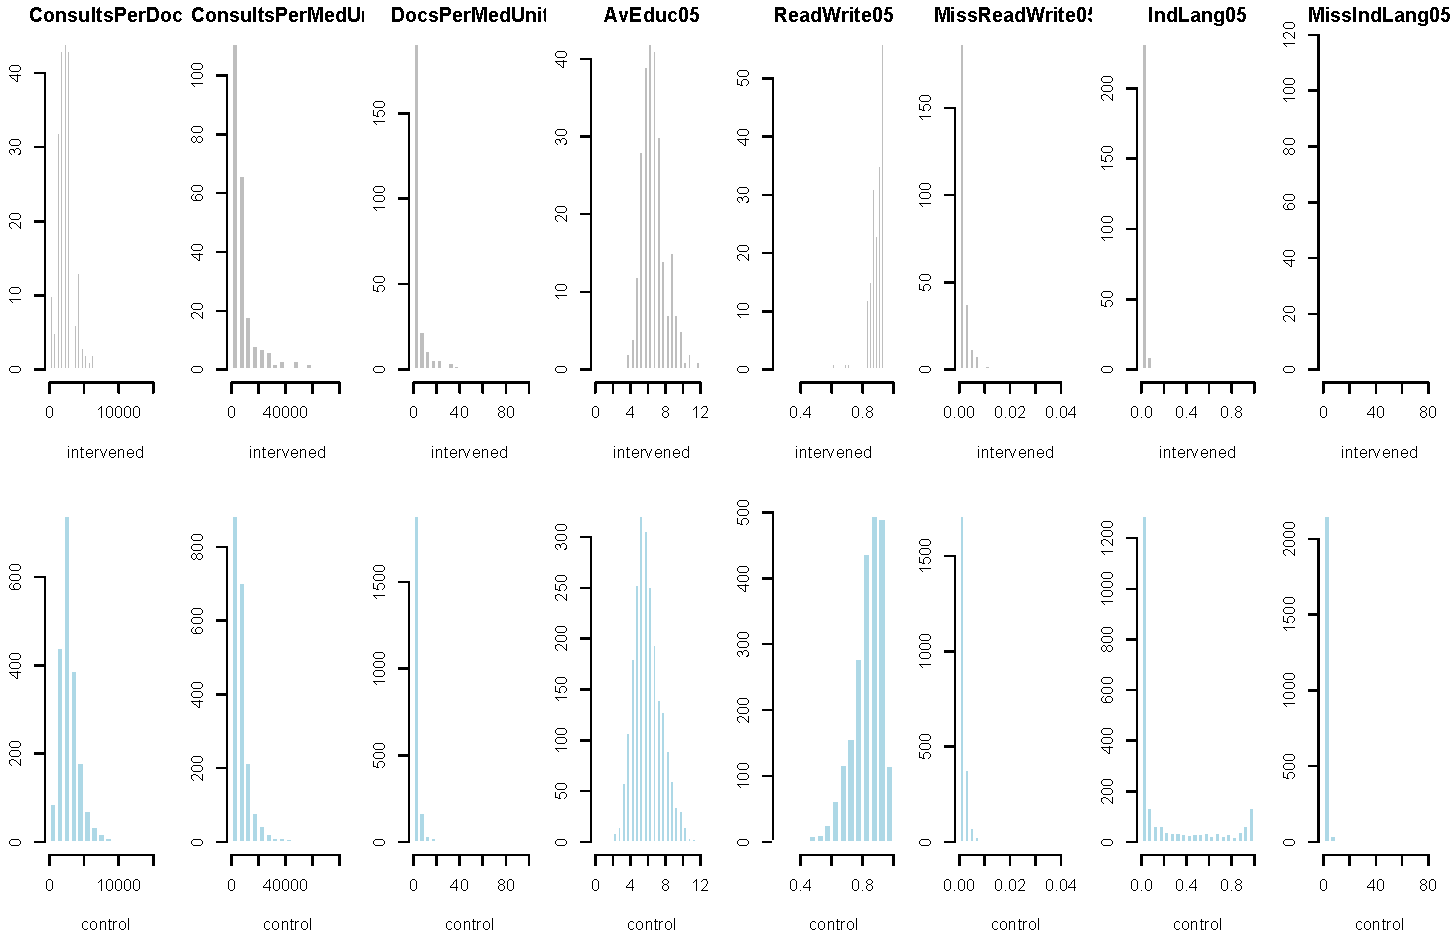
\includegraphics[scale=0.6]{InitBalance1.pdf}
\caption{Histograms to compare distributions in original pools.}
\label{initBalance1}
\end{figure}

\begin{figure}[ht]

    \centering
        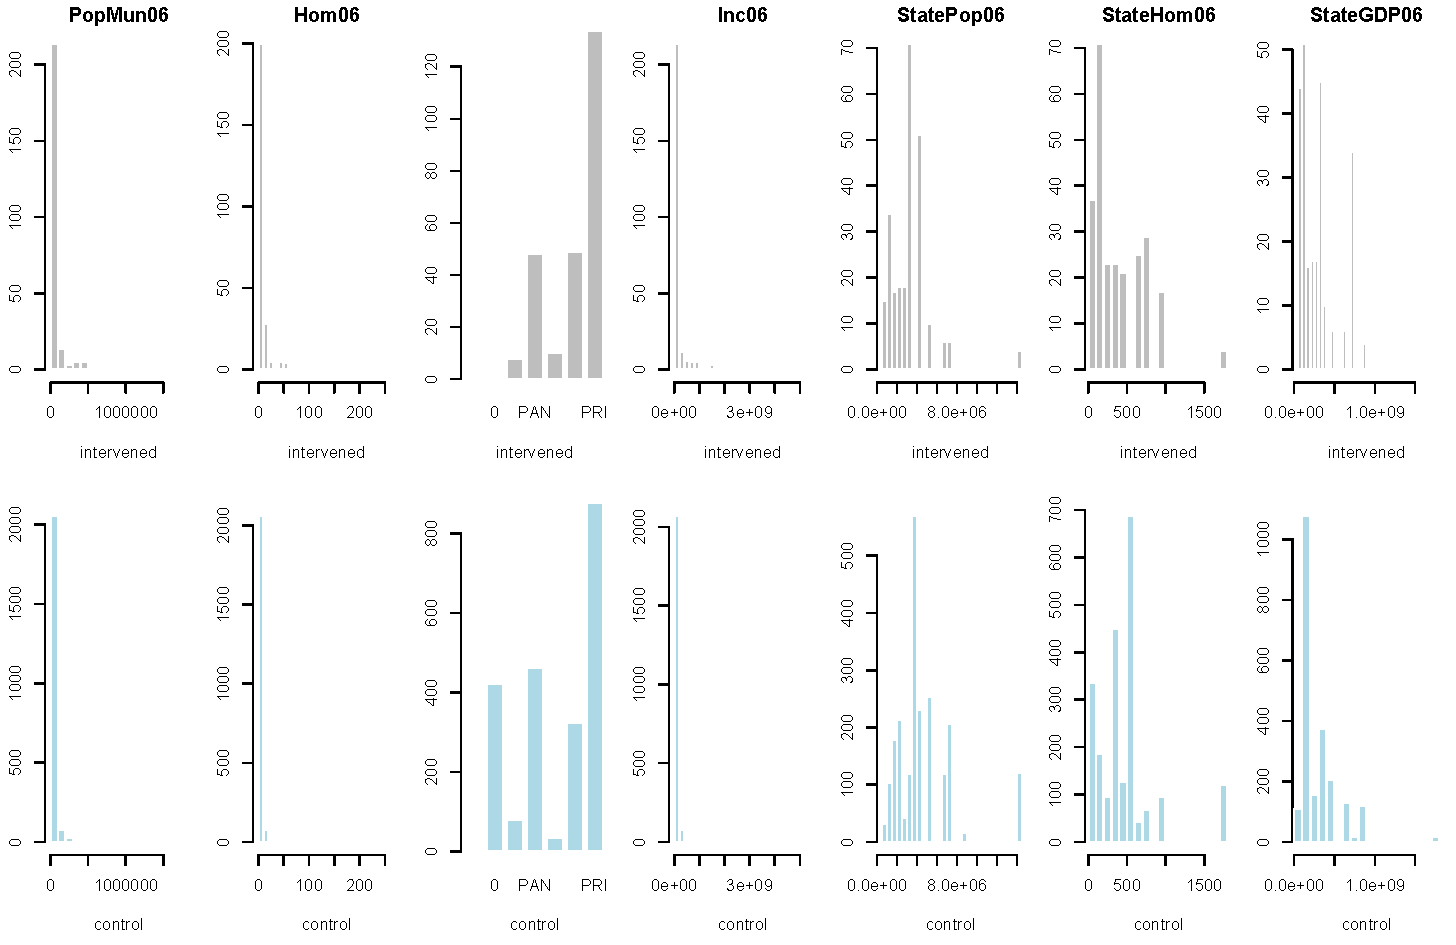
\includegraphics[scale=0.6]{InitBalance2.pdf}
\caption{Histograms and Barplots  to compare distributions in original pools.}
\label{initBalance2}
\end{figure}

We further explore the overlap for homicides
\begin{figure}[ht]

    \centering
        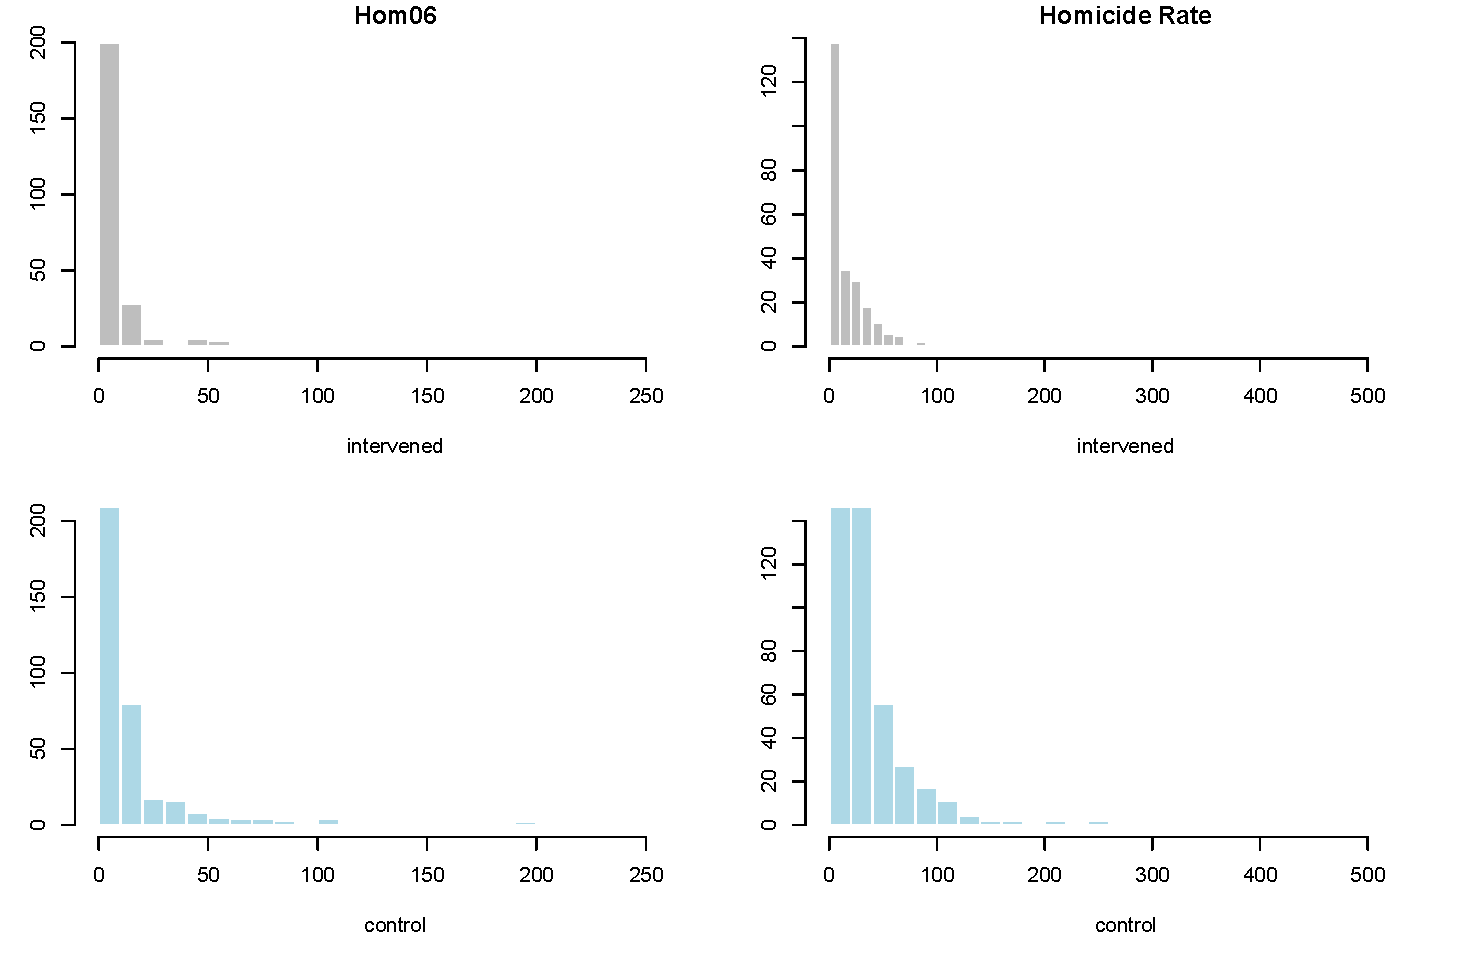
\includegraphics[scale=0.6]{ZoomHom.pdf}
\caption{Zooming in to Homicide Rate}
\label{ZoomHom}
\end{figure}

In some tries of matching we observe that the major imbalance is at the `Homicide 2006' covariate (should we have homicide rate or do the weights take care of that?)



\begin{figure}[ht]
    \centering
        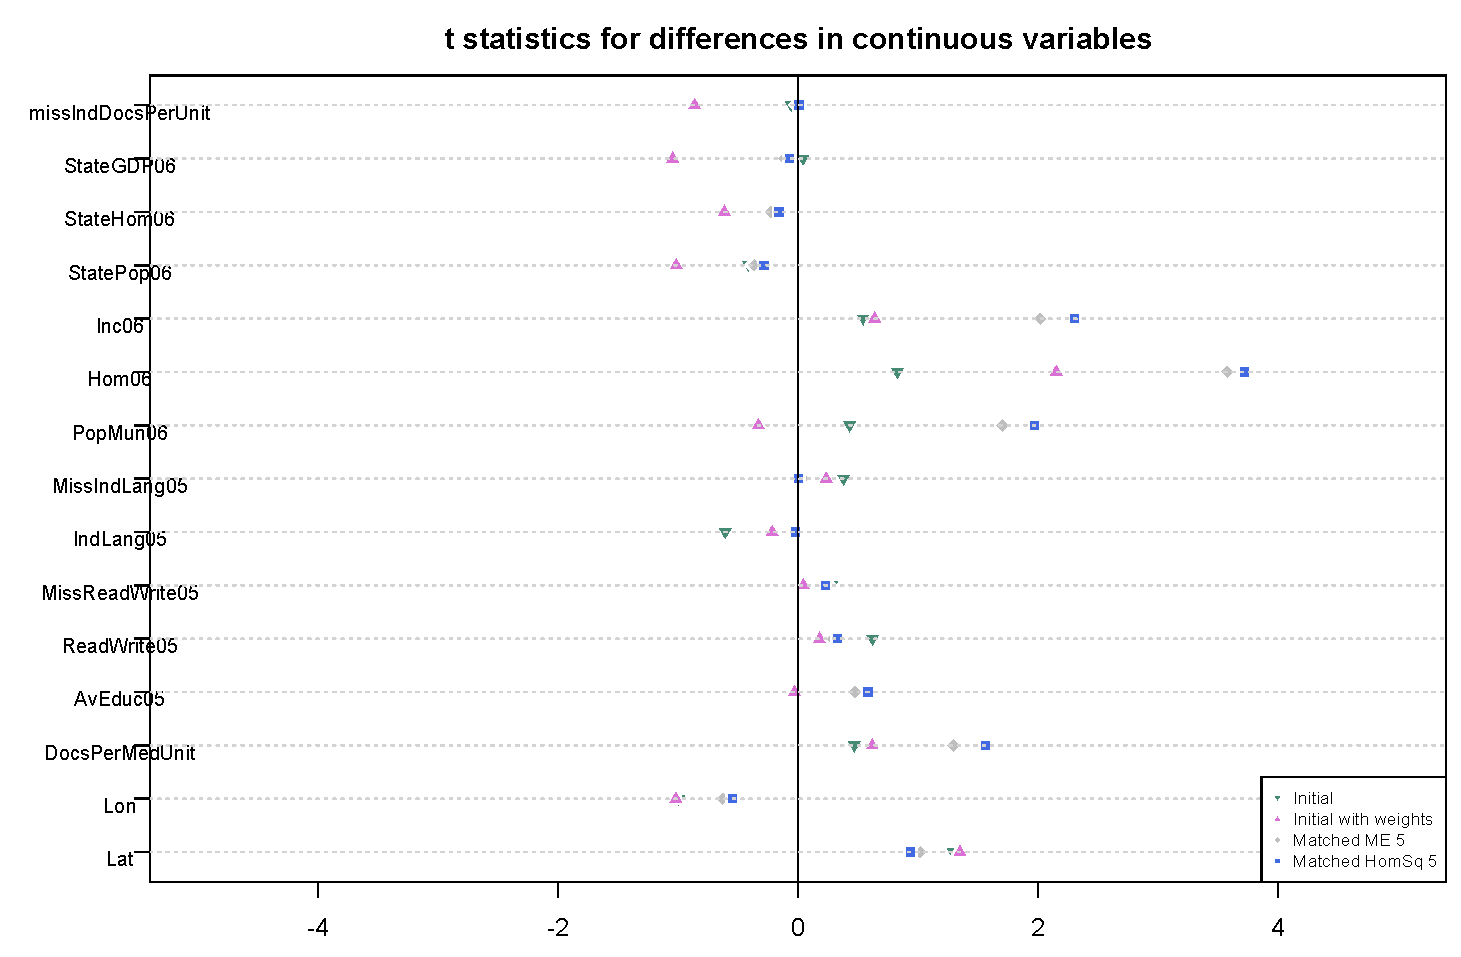
\includegraphics[scale=0.5]{MEloveplot.pdf}
\end{figure}

\section{Comments}
Perhaps a more comprehensive way of approaching this problem is to analyze the homicide rate time series using Synthetic Matching.

	
\end{document}